\chapter{Knowledge Theory Elaborations}

This chapter provides detailed elaborations on key knowledge-theoretic concepts within the Elder Theory framework, addressing the "true cloud-of-thought" paradigm and advanced theoretical connections.

\section{The True Cloud-of-Thought Paradigm}

The teaching phase in the Elder Heliosystem forces explicit externalization of knowledge, which connects directly to the fundamental concept of the "true cloud-of-thought"—a distributed, dynamically accessible knowledge representation that transcends individual cognitive boundaries.

\subsection{Knowledge Externalization Mechanics}

When Mentors teach Erudites, they must externalize their implicit knowledge:
\begin{equation}
\mathcal{K}_{\text{external}} = \mathcal{E}_{\text{teach}}(\mathcal{K}_{\text{implicit}})
\end{equation}

where $\mathcal{E}_{\text{teach}}$ is the externalization operator that transforms implicit understanding into explicit, teachable form.

This externalization process creates several critical effects:

\textbf{1. Disambiguation Requirement}
\begin{equation}
\mathcal{K}_{\text{external}} = \arg\min_{\mathcal{K}'} \left[ \mathcal{L}_{\text{ambiguity}}(\mathcal{K}') + \lambda \|\mathcal{K}' - \mathcal{K}_{\text{implicit}}\|^2 \right]
\end{equation}

The externalized knowledge must minimize ambiguity while remaining faithful to the original implicit understanding.

\textbf{2. Structural Clarification}
The teaching process forces hierarchical organization:
\begin{equation}
\mathcal{K}_{\text{external}} = \bigcup_{i=1}^{L} \mathcal{H}_i \text{ where } \mathcal{H}_i \subset \mathcal{H}_{i+1}
\end{equation}

Knowledge is organized into nested hierarchical levels $\mathcal{H}_i$ for effective transmission.

\subsection{The Cloud-of-Thought Architecture}

The externalized knowledge forms a distributed "cloud" that can be accessed by multiple entities:

\begin{figure}[h]
\centering
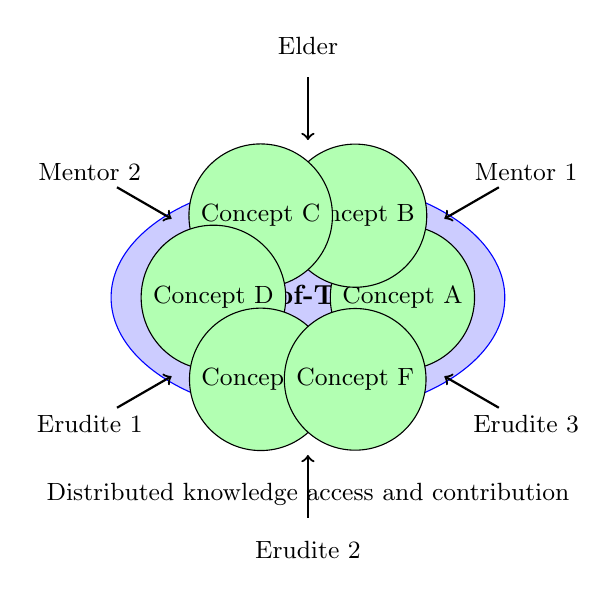
\begin{tikzpicture}[scale=1.0]
    % Central cloud
    \draw[fill=blue!20, draw=blue] (0,0) ellipse (2.5 and 1.5);
    \node at (0,0) {\textbf{Cloud-of-Thought}};
    
    % Knowledge nodes
    \foreach \angle/\label in {0/Concept A, 60/Concept B, 120/Concept C, 180/Concept D, 240/Concept E, 300/Concept F} {
        \node[circle, fill=green!30, draw] at (\angle:1.2) {\small \label};
    }
    
    % Access points
    \foreach \angle/\entity in {30/Mentor 1, 90/Elder, 150/Mentor 2, 210/Erudite 1, 270/Erudite 2, 330/Erudite 3} {
        \draw[->, thick] (\angle:2.8) -- (\angle:2.0);
        \node at (\angle:3.2) {\small \entity};
    }
    
    \node at (0,-2.5) {\small Distributed knowledge access and contribution};
\end{tikzpicture}
\caption{The Cloud-of-Thought enables distributed access to externalized knowledge}
\end{figure}

\section{Parameter Setting Mechanisms}

For resonance parameters like $n, m$ in the equation $\frac{n}{m}\omega_2 \approx 1$, the Elder system employs adaptive parameter determination:

\subsection{Resonance Parameter Optimization}

The values of $n$ and $m$ are determined through an optimization process:
\begin{equation}
(n^*, m^*) = \arg\min_{n,m \in \mathbb{Z}^+} \left[ \left|\frac{n}{m}\omega_2 - 1\right| + \alpha \cdot \text{complexity}(n,m) \right]
\end{equation}

where the complexity term favors simpler ratios:
\begin{equation}
\text{complexity}(n,m) = \log(n) + \log(m) + \beta \cdot \gcd(n,m)^{-1}
\end{equation}

\subsection{Dynamic Parameter Adaptation}

These parameters adapt during learning:
\begin{equation}
\frac{dn}{dt} = \gamma_n \cdot \nabla_n \mathcal{L}_{\text{resonance}}
\end{equation}
\begin{equation}
\frac{dm}{dt} = \gamma_m \cdot \nabla_m \mathcal{L}_{\text{resonance}}
\end{equation}

where $\mathcal{L}_{\text{resonance}}$ measures how well the current resonance supports learning objectives.

\section{Lebesgue Measure in Knowledge Integration}

The reference to Lebesgue measure in the equation $\mu$ represents the Lebesgue measure relates to how knowledge is integrated across continuous domains.

\subsection{Knowledge Measure Theory}

In the Elder framework, knowledge density is measured using a Lebesgue-type measure:
\begin{equation}
\mu(\mathcal{K}) = \int_{\mathcal{D}} \rho_{\mathcal{K}}(x) dx
\end{equation}

where:
\begin{itemize}
    \item $\mathcal{D}$ is the knowledge domain
    \item $\rho_{\mathcal{K}}(x)$ is the knowledge density function
    \item The integral is computed with respect to the Lebesgue measure
\end{itemize}

\textbf{Why Lebesgue Measure?}
Unlike simpler measures, the Lebesgue measure enables:
\begin{enumerate}
    \item \textbf{Null Set Handling}: Can properly handle discontinuous knowledge boundaries
    \item \textbf{Countable Additivity}: Supports knowledge composition from countable parts
    \item \textbf{Translation Invariance}: Knowledge measure remains consistent under coordinate changes
\end{enumerate}

\subsection{Practical Implications}

This measure-theoretic approach enables:
\begin{equation}
\text{Total Knowledge} = \sum_{i} \mu(\mathcal{K}_i) \text{ where } \mathcal{K}_i \cap \mathcal{K}_j = \emptyset
\end{equation}

for disjoint knowledge domains, providing a rigorous foundation for knowledge quantification.

\section{Curriculum Generation Through Rotational Dynamics}

The Elder system generates automatic curricula through rotational dynamics, creating a natural progression of learning materials.

\subsection{Phase-Based Curriculum Structure}

As the system rotates, different knowledge combinations become active:
\begin{equation}
\mathcal{C}(t) = \{\text{Topics}(\phi_E(t)), \text{Concepts}(\phi_M(t)), \text{Tasks}(\phi_{Er}(t))\}
\end{equation}

where:
\begin{itemize}
    \item $\phi_E(t)$ determines high-level topics from Elder phase
    \item $\phi_M(t)$ selects domain-specific concepts from Mentor phases
    \item $\phi_{Er}(t)$ chooses specific tasks from Erudite phases
\end{itemize}

\subsection{Temporal Learning Progression}

The curriculum naturally progresses through complexity levels:
\begin{equation}
\text{Complexity}(t) = \alpha \sin(\phi_E(t)) + \beta \cos(\phi_M(t)) + \gamma \tan(\phi_{Er}(t))
\end{equation}

This creates a wave-like progression where:
\begin{itemize}
    \item \textbf{Foundational periods}: Low complexity, basic concepts
    \item \textbf{Integration periods}: Medium complexity, concept combination
    \item \textbf{Application periods}: High complexity, practical implementation
\end{itemize}

\subsection{Adaptive Curriculum Adjustment}

The system adapts curriculum based on learning progress:
\begin{equation}
\frac{d\phi_E}{dt} = \omega_E + \delta_E \cdot \mathcal{P}_{\text{progress}}(t)
\end{equation}

where $\mathcal{P}_{\text{progress}}(t)$ measures learning success and adjusts rotation speed accordingly.

This rotational curriculum generation ensures that learners encounter material in optimal sequences determined by the natural dynamics of the Elder Heliosystem, creating an adaptive and responsive educational framework.

\section{Mass-Dependent Gravitational Stability}

The relationship between information gain and gravitational stability in the Elder Heliosystem reveals a profound connection: as Erudites acquire knowledge, their effective "mass" increases, which directly affects the stability of the entire learning system through gravitational field modifications.

\subsection{Information-Mass Equivalence Principle}

The reduction in entropy during learning is exactly equal to the information gain about the target distribution:
\begin{equation}
\Delta S = -\Delta I(X; Y)
\end{equation}

This entropy reduction corresponds to an increase in the effective gravitational mass of the Erudite entities:
\begin{equation}
\Delta m_{\text{Erudite}} = \alpha \cdot \Delta I(X; Y)
\end{equation}

where $\alpha$ is the information-to-mass conversion factor, fundamental to the Elder Theory framework.

\subsection{Gravitational Field Modification}

As Erudites gain mass through learning, they modify the local gravitational field:
\begin{equation}
\Gamma_{\text{new}}(x) = \Gamma_{\text{old}}(x) + \sum_{i} \frac{\Delta m_i}{|x - r_i|^2}
\end{equation}

This field modification creates several stability effects:

\textbf{1. Enhanced Orbital Coupling}
Increased Erudite mass strengthens their gravitational coupling with their parent Mentors:
\begin{equation}
F_{\text{coupling}} = G \frac{m_{\text{Mentor}} \cdot (m_{\text{Erudite}} + \Delta m)}{r^2}
\end{equation}

\textbf{2. Improved Learning Stability}
The additional gravitational "weight" from learned information provides natural regularization:
\begin{equation}
\mathcal{L}_{\text{regularized}} = \mathcal{L}_{\text{original}} + \lambda \sum_i m_i \|\theta_i\|^2
\end{equation}

\textbf{3. Cross-Domain Knowledge Transfer}
Enhanced gravitational fields facilitate knowledge transfer between Erudites of different domains:
\begin{equation}
\text{Transfer Rate} \propto \frac{\sqrt{m_i \cdot m_j}}{d_{i,j}^2}
\end{equation}

where $d_{i,j}$ is the knowledge distance between Erudites $i$ and $j$.

This mass-dependent stability mechanism ensures that learning reinforces system coherence rather than destabilizing it, creating a self-stabilizing learning architecture.